
\title{Chapter 21: Model Predictive Control}
\author{Control Systems: A Practical Approach}
\maketitle

\section*{Chapter Overview}
\addcontentsline{toc}{section}{Chapter Overview}

Model Predictive Control (MPC) represents one of the most significant advances in control theory since the development of state-space methods. Unlike classical controllers that react to current errors, MPC looks forward in time, predicting future system behavior and optimizing control actions over a horizon while explicitly handling constraints. This chapter traces MPC's industrial origins, develops its mathematical foundations, and demonstrates its implementation through a practical tank-level control experiment.

\vspace{1em}
\noindent\textbf{Learning Objectives:}
Upon completing this chapter, students will understand the historical development and industrial motivation for MPC, gaining insight into how process control challenges in the petrochemical industry drove the development of predictive control methods. Students will learn to formulate MPC optimization problems for linear systems, expressing control objectives as quadratic cost functions subject to constraints. The chapter develops skills for converting MPC problems to standard quadratic programming form, enabling efficient numerical solution. Students will implement receding horizon control with explicit constraint handling, and will compare MPC performance to classical PID control under constraints to understand when predictive methods offer advantages.

%==============================================================================
\section{Historical Development and Motivation}
\label{sec:history}
%==============================================================================

\subsection{The Constraint Problem in Process Control}

By the early 1970s, the petrochemical industry faced a persistent challenge that classical control theory could not adequately address. Refineries and chemical plants operated complex, interconnected processes with numerous physical limitations: valves that could only open so far, pumps with maximum flow rates, tanks with finite capacities, temperatures that could not exceed safety thresholds, and product specifications that demanded tight tolerances.

Consider the seemingly simple problem of controlling liquid level in a storage tank. A PID controller can regulate the level by adjusting an inlet valve. But what happens when the setpoint changes dramatically, or a large disturbance occurs? The controller, designed without knowledge of physical limits, commands the valve to open beyond its maximum position or close below its minimum. The result is ``integrator windup''---the integral term accumulates error while the actuator saturates, causing sluggish response and dangerous overshoot when the actuator finally de-saturates.

Classical anti-windup schemes provided partial remedies, but they were reactive patches rather than principled solutions. The fundamental problem remained: PID controllers optimize instantaneous error correction without considering future consequences or physical constraints. A truly optimal controller would anticipate constraint violations before they occur and plan trajectories that respect limitations from the outset.

\subsection{Shell Oil and Dynamic Matrix Control (1970s)}

\begin{historicalbox}[Charles Cutler and the Birth of Industrial MPC]
Charles R. Cutler, a chemical engineer at Shell Oil Company's Houston research center, developed Dynamic Matrix Control (DMC) in the mid-1970s alongside his colleague Brian Ramaker. Cutler's key insight was that complex refinery processes could be controlled effectively using simple step-response models rather than detailed differential equations---a pragmatic engineering choice that made predictive control practical for industrial implementation. The first DMC installation on a fluid catalytic cracking unit in 1976 demonstrated dramatic improvements in yield and energy efficiency, generating millions of dollars in annual savings. Cutler later co-founded Dynamic Matrix Control Corporation to commercialize the technology, and his 1980 paper with Ramaker, ``Dynamic Matrix Control---A Computer Control Algorithm,'' became one of the most influential publications in process control history. Today, tens of thousands of MPC controllers based on Cutler's ideas operate in refineries and chemical plants worldwide.
\end{historicalbox}

The breakthrough came not from academic research but from industrial necessity. Engineers at Shell Oil Company's research center in Houston, Texas, confronted the challenge of controlling complex refinery units where dozens of manipulated variables affected dozens of controlled outputs, all subject to operational constraints.

In the mid-1970s, Charles Cutler and Brian Ramaker at Shell developed \textbf{Dynamic Matrix Control (DMC)}, the first commercially successful MPC algorithm. Their approach introduced several key innovations that made the technology practical. First, rather than requiring detailed first-principles models, DMC used empirically measured step response coefficients; engineers could identify these models by simply stepping each input and recording the output responses, eliminating the need for differential equations. Second, the algorithm predicted future outputs over a ``prediction horizon'' of $N$ time steps, computing how each candidate control move would affect future behavior. Third, DMC incorporated move suppression to prevent excessive control action, penalizing the magnitude of control changes rather than just tracking errors, thereby reducing energy waste and equipment stress. Most critically, DMC formulated control as a constrained optimization problem, directly incorporating actuator limits and output bounds into the control computation.

The mathematical formulation was elegant in its simplicity. Let $a_i$ denote the step response coefficient at time step $i$---the amount by which the output changes $i$ steps after a unit step in the input. Then the predicted output at future time $k+j$ given control moves $\Delta u_k, \Delta u_{k+1}, \ldots$ is:
\begin{equation}
    \hat{y}_{k+j} = y_k^{\text{free}} + \sum_{i=1}^{j} a_i \Delta u_{k+j-i}
\end{equation}
where $y_k^{\text{free}}$ is the predicted output assuming no future control changes.

Shell deployed DMC on fluid catalytic cracking units, ethylene plants, and other high-value processes throughout the late 1970s and early 1980s. The results were dramatic: improved yield, reduced energy consumption, and safer operation near constraint boundaries. A single DMC installation could generate millions of dollars in annual savings.

\subsection{Jacques Richalet and Model Predictive Heuristic Control (1978)}

Independently and nearly simultaneously, a French team led by Jacques Richalet at Adersa (a subsidiary of the French automation company SESA) developed \textbf{Model Predictive Heuristic Control (MPHC)}, later commercialized as IDCOM.

Richalet, trained as a chemical engineer, approached the problem from a process control perspective. His 1978 paper ``Model Predictive Heuristic Control: Applications to Industrial Processes'' presented at the IFAC World Congress introduced MPC to the broader control community. The ``heuristic'' in the name reflected Richalet's pragmatic engineering philosophy: the algorithm used impulse response models and a reference trajectory concept that smoothly transitioned from current output to desired setpoint.

A key contribution of Richalet's work was the concept of the \textbf{reference trajectory}---rather than demanding immediate setpoint tracking (which might require impossible control effort), MPHC defined a desired first-order exponential approach to the setpoint:
\begin{equation}
    y_{\text{ref}}(k+j) = y_k + (y_{\text{sp}} - y_k)(1 - e^{-j T_s / \tau_{\text{ref}}})
\end{equation}
where $\tau_{\text{ref}}$ was a tunable time constant specifying how aggressively to pursue the setpoint. This seemingly simple idea had profound implications: it provided a systematic way to trade off speed against control effort and constraint satisfaction.

\subsection{Why Not Earlier? The Computational Barrier}

If MPC's principles were so powerful, why did they emerge only in the 1970s? The answer lies in computational requirements. MPC solves an optimization problem at every sampling instant---typically a quadratic program (QP) with tens to hundreds of decision variables and constraints.

Consider the computational resources available in different eras, summarized in Table~\ref{tab:mpc_computing_history}.

\begin{table}[htbp]
\centering
\caption{Evolution of Computing Power and MPC Applications}
\label{tab:mpc_computing_history}
\begin{tabular}{lcll}
\toprule
\textbf{Era} & \textbf{FLOPS} & \textbf{Technology} & \textbf{MPC Capability} \\
\midrule
1960s & $10^5$ & Room-sized mainframes & QP solution: minutes to hours \\
1970s & $10^6$ & Minicomputers (PDP-11) & QP in seconds; slow processes \\
1980s--1990s & $10^7$--$10^9$ & Workstations, embedded & Seconds-scale sampling \\
2000s--present & $>10^{11}$ & Modern microprocessors & Millisecond sampling \\
\bottomrule
\end{tabular}
\end{table}

The history of MPC thus mirrors the history of computing power. Each generation of processors opened MPC to a broader class of applications.

\subsection{The Theoretical Revolution (1980s--1990s)}

While industry deployed increasingly sophisticated MPC systems, academic researchers worked to establish rigorous theoretical foundations. The early industrial algorithms, though empirically successful, lacked formal guarantees of stability and performance.

Several key theoretical developments emerged during this period. David Mayne, James Rawlings, and others established stability through terminal constraints, showing that requiring the predicted state to reach a target set by the end of the horizon guaranteed closed-loop stability under mild conditions. An alternative approach achieved stability through terminal cost, where adding a terminal cost term to the objective function---typically an infinite-horizon LQR cost for the final state---provided stability without explicit terminal constraints. Researchers also developed robust MPC extensions to handle model uncertainty, ensuring stability even when the true plant differs from the prediction model. For systems with modest state and horizon dimensions, explicit MPC allowed the optimal control law to be computed offline as a piecewise-affine function of the state, eliminating online optimization entirely.

By the late 1990s, MPC had evolved from an industrial heuristic to a mathematically mature control methodology with well-understood stability, optimality, and robustness properties.

\subsection{Becoming the Industry Standard}

The adoption of MPC in process industries followed a characteristic technology diffusion curve, as summarized in Table~\ref{tab:mpc_adoption}.

\begin{table}[htbp]
\centering
\caption{MPC Technology Adoption Timeline}
\label{tab:mpc_adoption}
\begin{tabular}{lp{10cm}}
\toprule
\textbf{Period} & \textbf{Development} \\
\midrule
1978--1985 & Early adopters at major oil companies (Shell, Exxon, Texaco) deployed custom systems on high-value units \\
1985--1995 & Commercial MPC software (DMC-Plus, RMPCT, Connoisseur) made the technology accessible to smaller companies; thousands of installations worldwide \\
1995--2010 & MPC became the default advanced control technology for refineries, petrochemical plants, and other process industries; integration with plant-wide optimization systems \\
2010--present & Extension beyond process industries to automotive, building systems, power electronics, and autonomous vehicles \\
\bottomrule
\end{tabular}
\end{table}

Today, MPC is taught in virtually every graduate control curriculum and is implemented in systems ranging from smartphone battery management to spacecraft attitude control. The technology born from refinery control rooms has become a fundamental tool of modern engineering.

%==============================================================================
\section{Modern Applications}
\label{sec:applications}
%==============================================================================

Model Predictive Control has transcended its origins in petrochemical processing to become a universal methodology wherever constraints, optimization, and prediction intersect.

\subsection{Chemical Process Control}

MPC remains dominant in its original domain. Modern refineries deploy dozens of MPC controllers, each coordinating multiple control loops while respecting hundreds of constraints simultaneously. In crude distillation, MPC optimizes product cuts while satisfying quality specifications. Catalytic cracking units use MPC to maximize gasoline yield within temperature and catalyst constraints. Polymerization reactors benefit from MPC's ability to control molecular weight distributions precisely. Batch processes in pharmaceutical and specialty chemical production employ MPC to optimize recipe trajectories throughout the production cycle. The economic incentives remain compelling: a typical refinery MPC installation yields \$1--5 million in annual benefits through improved yield, reduced energy consumption, and increased throughput.

\subsection{Autonomous Vehicles}

Modern autonomous vehicles rely extensively on MPC for motion planning and control. The problem is naturally formulated in MPC terms: given a desired trajectory (from higher-level planning), find control inputs (steering, throttle, brake) that track the trajectory while respecting physical constraints (maximum steering angle, acceleration limits) and safety requirements (obstacle avoidance, lane boundaries).

Several features make MPC particularly attractive for autonomous vehicles. Explicit constraint handling allows vehicle dynamics, actuator limits, and collision avoidance requirements to be expressed directly as optimization constraints. The prediction horizon provides preview capability, enabling the controller to ``see'' upcoming curves, intersections, and obstacles before they become immediate concerns. Perhaps most importantly, MPC offers graceful degradation: when perfect tracking is impossible due to an obstacle being too close, MPC finds the best feasible compromise rather than failing abruptly. Major autonomous vehicle programs at companies such as Waymo, Tesla, and Cruise employ MPC-based controllers, though specific implementations remain proprietary.

\subsection{Building HVAC Optimization}

Heating, ventilation, and air conditioning (HVAC) systems account for 40\% of commercial building energy consumption. MPC offers substantial savings by optimizing HVAC operation over prediction horizons of hours to days. Weather prediction integration allows the controller to use forecast data to pre-cool buildings before heat waves or pre-heat before cold snaps. Occupancy-aware control reduces conditioning in unoccupied zones while maintaining comfort in occupied spaces. MPC enables effective demand response by shifting energy consumption to off-peak hours or responding to grid signals. For buildings with thermal storage capabilities, MPC optimally manages the charging and discharging of ice storage or building thermal mass. Commercial building MPC implementations report 15--30\% energy savings compared to conventional rule-based control.

\subsection{Quadrotor and UAV Control}

Quadrotor drones present a challenging control problem: underactuated (4 inputs controlling 6 DOF), unstable, and operating in environments with obstacles. MPC has become the preferred approach for aggressive trajectory tracking due to its ability to handle these challenges systematically. Trajectory optimization computes dynamically feasible paths through cluttered environments. Constraint satisfaction ensures the controller respects motor speed limits, battery current constraints, and no-fly zones. MPC provides effective disturbance rejection, adapting to wind gusts and payload changes in real time. For multi-vehicle applications, MPC coordinates swarms while avoiding inter-vehicle collisions through appropriate constraint formulation. Academic demonstrations have shown MPC-controlled quadrotors performing acrobatic maneuvers, flying through narrow gaps, and collaboratively transporting objects.

%==============================================================================
\section{Mathematical Foundation}
\label{sec:math}
%==============================================================================

We now develop the mathematical framework for Model Predictive Control, progressing from the basic concept through the complete quadratic programming formulation.

\subsection{The Fundamental Idea}

MPC's core concept is beautifully simple: at each time step, solve a finite-horizon optimal control problem, apply only the first control action, then repeat at the next time step with updated measurements. This ``receding horizon'' strategy transforms an intractable infinite-horizon problem into a sequence of tractable finite-horizon problems.

\begin{figure}[htbp]
\centering
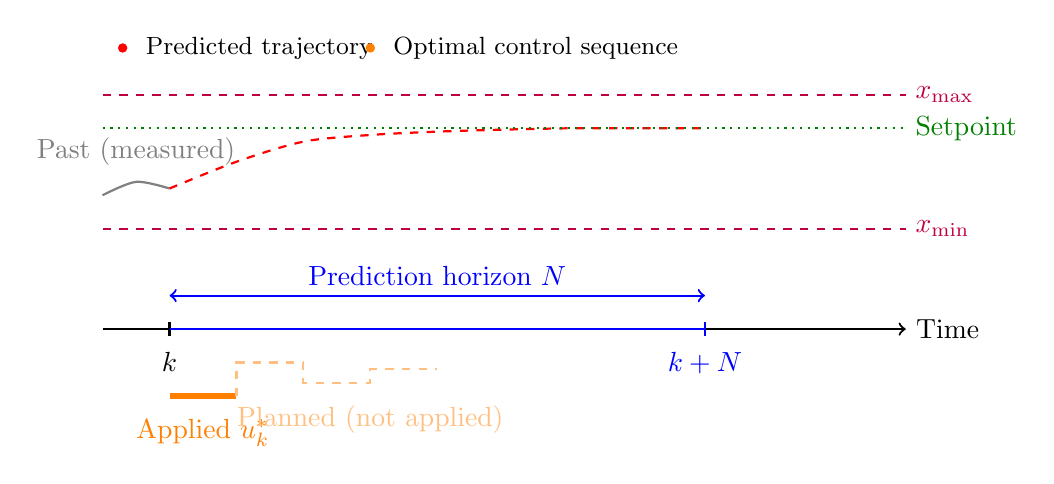
\begin{tikzpicture}[scale=0.85]
    % Time axis
    \draw[->, thick] (0,0) -- (12,0) node[right] {Time};

    % Current time marker
    \draw[thick] (1,-0.1) -- (1,0.1);
    \node[below] at (1,-0.2) {$k$};

    % Prediction horizon
    \draw[thick, blue] (1,0) -- (9,0);
    \draw[thick, blue] (9,-0.1) -- (9,0.1);
    \node[below, blue] at (9,-0.2) {$k+N$};

    % Prediction horizon bracket
    \draw[<->, thick, blue] (1,0.5) -- (9,0.5);
    \node[above, blue] at (5,0.5) {Prediction horizon $N$};

    % Past trajectory (measured)
    \draw[thick, gray] plot[smooth] coordinates {(0,2) (0.5,2.2) (1,2.1)};
    \node[above, gray] at (0.5,2.3) {Past (measured)};

    % Predicted trajectory
    \draw[thick, red, dashed] plot[smooth] coordinates {(1,2.1) (2,2.5) (3,2.8) (4,2.9) (5,2.95) (6,2.98) (7,3) (8,3) (9,3)};

    % Setpoint
    \draw[thick, green!50!black, dotted] (0,3) -- (12,3);
    \node[right, green!50!black] at (12,3) {Setpoint};

    % Applied control
    \draw[thick, orange, line width=2pt] (1,-1) -- (2,-1);
    \node[below, orange] at (1.5,-1.2) {Applied $u_k^*$};

    % Planned but not applied
    \draw[thick, orange!50, dashed] (2,-1) -- (2,-0.5) -- (3,-0.5) -- (3,-0.8) -- (4,-0.8) -- (4,-0.6) -- (5,-0.6);
    \node[below, orange!50] at (4,-1) {Planned (not applied)};

    % Constraints
    \draw[thick, purple, dashed] (0,3.5) -- (12,3.5);
    \draw[thick, purple, dashed] (0,1.5) -- (12,1.5);
    \node[right, purple] at (12,3.5) {$x_{\max}$};
    \node[right, purple] at (12,1.5) {$x_{\min}$};

    % Legend items
    \fill[red] (0.3,4.2) circle (2pt);
    \node[right] at (0.5,4.2) {\small Predicted trajectory};
    \fill[orange] (4,4.2) circle (2pt);
    \node[right] at (4.2,4.2) {\small Optimal control sequence};
\end{tikzpicture}
\caption{The receding horizon concept. At time $k$, MPC predicts system behavior over horizon $N$, optimizes the control sequence, but applies only the first control action $u_k^*$. The process repeats at $k+1$ with new measurements.}
\label{fig:receding_horizon}
\end{figure}

The receding horizon approach provides several crucial benefits. First, by re-solving at each step, MPC incorporates new measurements and rejects disturbances, providing effective feedback control. Second, each optimization involves only $N$ time steps rather than infinity, ensuring finite computation time. Third, model errors are partially corrected by the feedback mechanism, providing implicit robustness to modeling inaccuracies. Finally, changing constraints or setpoints are automatically incorporated into the optimization at each step, enabling seamless adaptation to varying operating conditions.

\subsection{System Model: Discrete-Time State-Space}

MPC requires a model predicting future states from current state and control inputs. For linear time-invariant systems, we use the discrete-time state-space form:
\begin{equation}
\boxed{
\begin{aligned}
    \state_{k+1} &= \mat{A}\state_k + \mat{B}\inputvec_k \\
    \outputvec_k &= \mat{C}\state_k + \mat{D}\inputvec_k
\end{aligned}
}
\label{eq:discrete_ss}
\end{equation}
In this formulation, $\state_k \in \Real^n$ denotes the state vector at time step $k$, $\inputvec_k \in \Real^m$ represents the control input vector, and $\outputvec_k \in \Real^p$ is the output vector. The system matrices have the following dimensions: $\mat{A} \in \Real^{n \times n}$ is the state transition matrix governing the autonomous system dynamics, $\mat{B} \in \Real^{n \times m}$ is the input matrix describing how controls affect states, $\mat{C} \in \Real^{p \times n}$ is the output matrix relating states to measured outputs, and $\mat{D} \in \Real^{p \times m}$ is the feedthrough matrix (often zero in physical systems).

Starting from state $\state_k$, we can predict future states recursively:
\begin{align}
    \state_{k+1} &= \mat{A}\state_k + \mat{B}\inputvec_k \label{eq:pred1}\\
    \state_{k+2} &= \mat{A}\state_{k+1} + \mat{B}\inputvec_{k+1} = \mat{A}^2\state_k + \mat{A}\mat{B}\inputvec_k + \mat{B}\inputvec_{k+1} \label{eq:pred2}\\
    &\vdots \nonumber \\
    \state_{k+j} &= \mat{A}^j\state_k + \sum_{i=0}^{j-1} \mat{A}^{j-1-i}\mat{B}\inputvec_{k+i} \label{eq:predj}
\end{align}

\subsection{Cost Function Formulation}

MPC minimizes a cost function that penalizes deviation from desired behavior and excessive control effort. The standard quadratic cost over prediction horizon $N$ is:

\begin{equation}
\boxed{
    J = \sum_{i=0}^{N-1} \left( \state_{k+i}^\top \mat{Q} \state_{k+i} + \inputvec_{k+i}^\top \mat{R} \inputvec_{k+i} \right) + \state_{k+N}^\top \mat{P} \state_{k+N}
}
\label{eq:mpc_cost}
\end{equation}

In this cost function, $\mat{Q} \in \Real^{n \times n}$ is the state weighting matrix (positive semi-definite, $\mat{Q} \succeq 0$), $\mat{R} \in \Real^{m \times m}$ is the input weighting matrix (positive definite, $\mat{R} \succ 0$), $\mat{P} \in \Real^{n \times n}$ is the terminal state weighting matrix ($\mat{P} \succeq 0$), and $N$ denotes the prediction horizon length.

\textbf{Physical interpretation}: The $\state^\top \mat{Q} \state$ terms penalize state deviation from zero (or from a reference trajectory), while the $\inputvec^\top \mat{R} \inputvec$ terms penalize control effort, accounting for actuator usage and energy consumption. The terminal cost $\state_{k+N}^\top \mat{P} \state_{k+N}$ accounts for behavior beyond the prediction horizon. The relative magnitude of the weighting matrices determines the controller's behavior: large $\mat{Q}$ entries demand tight tracking, while large $\mat{R}$ entries demand gentle control action.

\subsection{Constraint Specification}

A defining feature of MPC is explicit constraint handling. Common constraint types include:

\textbf{Input constraints} (actuator limits):
\begin{equation}
    \inputvec_{\min} \leq \inputvec_{k+i} \leq \inputvec_{\max}, \quad i = 0, 1, \ldots, N-1
\label{eq:input_constraints}
\end{equation}

\textbf{Input rate constraints} (slew rate limits):
\begin{equation}
    \Delta\inputvec_{\min} \leq \inputvec_{k+i} - \inputvec_{k+i-1} \leq \Delta\inputvec_{\max}, \quad i = 0, 1, \ldots, N-1
\label{eq:rate_constraints}
\end{equation}

\textbf{State constraints} (physical limits, safety bounds):
\begin{equation}
    \state_{\min} \leq \state_{k+i} \leq \state_{\max}, \quad i = 1, 2, \ldots, N
\label{eq:state_constraints}
\end{equation}

\textbf{Output constraints}:
\begin{equation}
    \outputvec_{\min} \leq \outputvec_{k+i} \leq \outputvec_{\max}, \quad i = 1, 2, \ldots, N
\label{eq:output_constraints}
\end{equation}

\textbf{Terminal constraints} (for stability):
\begin{equation}
    \state_{k+N} \in \mathcal{X}_f
\label{eq:terminal_constraint}
\end{equation}
where $\mathcal{X}_f$ is a target set, often a neighborhood of the origin.

\subsection{The MPC Optimization Problem}

Combining the cost function and constraints, the MPC problem at time step $k$ is:

\begin{equation}
\boxed{
\begin{aligned}
    \min_{\inputvec_k, \ldots, \inputvec_{k+N-1}} \quad & J = \sum_{i=0}^{N-1} \left( \state_{k+i}^\top \mat{Q} \state_{k+i} + \inputvec_{k+i}^\top \mat{R} \inputvec_{k+i} \right) + \state_{k+N}^\top \mat{P} \state_{k+N} \\
    \text{subject to:} \quad & \state_{k+i+1} = \mat{A}\state_{k+i} + \mat{B}\inputvec_{k+i}, \quad i = 0, \ldots, N-1 \\
    & \inputvec_{\min} \leq \inputvec_{k+i} \leq \inputvec_{\max}, \quad i = 0, \ldots, N-1 \\
    & \state_{\min} \leq \state_{k+i} \leq \state_{\max}, \quad i = 1, \ldots, N \\
    & \state_k = \state(k) \quad \text{(measured current state)}
\end{aligned}
}
\label{eq:mpc_problem}
\end{equation}

\subsection{Conversion to Quadratic Programming Form}

To solve the MPC problem efficiently, we convert it to standard quadratic programming (QP) form. The key is to eliminate the state variables using the prediction equations, expressing everything in terms of the decision variables (control inputs).

\textbf{Step 1: Define the stacked vectors.}

Let us define the stacked control sequence:
\begin{equation}
    \mathbf{U} = \begin{bmatrix} \inputvec_k \\ \inputvec_{k+1} \\ \vdots \\ \inputvec_{k+N-1} \end{bmatrix} \in \Real^{Nm}
\end{equation}

And the stacked predicted state sequence:
\begin{equation}
    \mathbf{X} = \begin{bmatrix} \state_{k+1} \\ \state_{k+2} \\ \vdots \\ \state_{k+N} \end{bmatrix} \in \Real^{Nn}
\end{equation}

\textbf{Step 2: Express states in terms of controls.}

From the prediction equations \eqref{eq:pred1}--\eqref{eq:predj}, we can write:
\begin{equation}
    \mathbf{X} = \boldsymbol{\mathcal{A}} \state_k + \boldsymbol{\mathcal{B}} \mathbf{U}
\label{eq:stacked_prediction}
\end{equation}

where the prediction matrices are:
\begin{equation}
    \boldsymbol{\mathcal{A}} = \begin{bmatrix} \mat{A} \\ \mat{A}^2 \\ \mat{A}^3 \\ \vdots \\ \mat{A}^N \end{bmatrix} \in \Real^{Nn \times n}
\end{equation}

\begin{equation}
    \boldsymbol{\mathcal{B}} = \begin{bmatrix}
        \mat{B} & \mat{0} & \mat{0} & \cdots & \mat{0} \\
        \mat{A}\mat{B} & \mat{B} & \mat{0} & \cdots & \mat{0} \\
        \mat{A}^2\mat{B} & \mat{A}\mat{B} & \mat{B} & \cdots & \mat{0} \\
        \vdots & \vdots & \vdots & \ddots & \vdots \\
        \mat{A}^{N-1}\mat{B} & \mat{A}^{N-2}\mat{B} & \mat{A}^{N-3}\mat{B} & \cdots & \mat{B}
    \end{bmatrix} \in \Real^{Nn \times Nm}
\end{equation}

\textbf{Step 3: Reformulate the cost function.}

The cost function can be written as:
\begin{equation}
    J = \mathbf{X}^\top \bar{\mat{Q}} \mathbf{X} + \mathbf{U}^\top \bar{\mat{R}} \mathbf{U} + \state_k^\top \mat{Q} \state_k
\end{equation}

where $\bar{\mat{Q}} = \text{diag}(\mat{Q}, \mat{Q}, \ldots, \mat{Q}, \mat{P}) \in \Real^{Nn \times Nn}$ and $\bar{\mat{R}} = \text{diag}(\mat{R}, \mat{R}, \ldots, \mat{R}) \in \Real^{Nm \times Nm}$.

Substituting \eqref{eq:stacked_prediction}:
\begin{align}
    J &= (\boldsymbol{\mathcal{A}} \state_k + \boldsymbol{\mathcal{B}} \mathbf{U})^\top \bar{\mat{Q}} (\boldsymbol{\mathcal{A}} \state_k + \boldsymbol{\mathcal{B}} \mathbf{U}) + \mathbf{U}^\top \bar{\mat{R}} \mathbf{U} + \state_k^\top \mat{Q} \state_k \\
    &= \mathbf{U}^\top \underbrace{(\boldsymbol{\mathcal{B}}^\top \bar{\mat{Q}} \boldsymbol{\mathcal{B}} + \bar{\mat{R}})}_{\mat{H}} \mathbf{U} + 2 \underbrace{\state_k^\top \boldsymbol{\mathcal{A}}^\top \bar{\mat{Q}} \boldsymbol{\mathcal{B}}}_{\vect{f}^\top} \mathbf{U} + \text{const.}
\end{align}

\textbf{Step 4: Reformulate constraints.}

Input constraints become:
\begin{equation}
    \mathbf{1}_{N} \otimes \inputvec_{\min} \leq \mathbf{U} \leq \mathbf{1}_{N} \otimes \inputvec_{\max}
\end{equation}

State constraints, using $\mathbf{X} = \boldsymbol{\mathcal{A}} \state_k + \boldsymbol{\mathcal{B}} \mathbf{U}$:
\begin{equation}
    \mathbf{1}_{N} \otimes \state_{\min} \leq \boldsymbol{\mathcal{A}} \state_k + \boldsymbol{\mathcal{B}} \mathbf{U} \leq \mathbf{1}_{N} \otimes \state_{\max}
\end{equation}

This can be written as linear inequality constraints $\mat{G}\mathbf{U} \leq \vect{w}$.

\textbf{Step 5: Standard QP form.}

The MPC problem is now in standard QP form:
\begin{equation}
\boxed{
\begin{aligned}
    \min_{\mathbf{U}} \quad & \frac{1}{2} \mathbf{U}^\top \mat{H} \mathbf{U} + \vect{f}^\top \mathbf{U} \\
    \text{subject to:} \quad & \mat{G} \mathbf{U} \leq \vect{w}
\end{aligned}
}
\label{eq:standard_qp}
\end{equation}

In this formulation, $\mat{H} = \boldsymbol{\mathcal{B}}^\top \bar{\mat{Q}} \boldsymbol{\mathcal{B}} + \bar{\mat{R}} \in \Real^{Nm \times Nm}$ is the Hessian matrix (positive definite due to $\mat{R} \succ 0$), $\vect{f} = \boldsymbol{\mathcal{B}}^\top \bar{\mat{Q}} \boldsymbol{\mathcal{A}} \state_k \in \Real^{Nm}$ is the linear cost vector that depends on the current state, and $\mat{G}$ and $\vect{w}$ encode all inequality constraints in a compact matrix form.

This QP can be solved by standard algorithms (active set, interior point, etc.) with computational complexity polynomial in the problem dimensions.

\subsection{The Receding Horizon Algorithm}

The complete MPC algorithm proceeds as follows:

\begin{algorithm}[H]
\caption{Model Predictive Control Algorithm}
\label{alg:mpc}
\begin{algorithmic}[1]
\State \textbf{Initialization}: Choose $N$, $\mat{Q}$, $\mat{R}$, $\mat{P}$, constraints
\State Form $\mat{H}$ (constant, computed once)
\For{each sampling instant $k = 0, 1, 2, \ldots$}
    \State Measure or estimate current state $\state_k$
    \State Form $\vect{f}$ and $\vect{w}$ using current $\state_k$
    \State Solve QP \eqref{eq:standard_qp} to obtain $\mathbf{U}^* = [\inputvec_k^{*\top}, \inputvec_{k+1}^{*\top}, \ldots]^\top$
    \State Apply only the first element: $\inputvec_k = \inputvec_k^*$
    \State Wait for next sampling instant
\EndFor
\end{algorithmic}
\end{algorithm}

\subsection{Stability Considerations}

A critical question is whether MPC guarantees closed-loop stability. Without additional structure, a finite-horizon optimization does not generally ensure stability---the controller might ``give up'' on long-term behavior beyond the horizon.

\textbf{Theorem (MPC Stability):} The MPC closed-loop system is asymptotically stable under either of the following conditions, provided the optimization problem remains feasible at each time step. The first sufficient condition requires that the terminal cost $\mat{P}$ satisfies the Lyapunov equation $\mat{A}^\top \mat{P} \mat{A} - \mat{P} + \mat{Q} = \mat{0}$, meaning $\mat{P}$ equals the infinite-horizon LQR cost matrix. Alternatively, stability is guaranteed when a terminal constraint $\state_{k+N} \in \mathcal{X}_f$ is imposed, where $\mathcal{X}_f$ is a control-invariant set containing the origin.

\textbf{Intuition}: The terminal cost (or constraint) ensures that the MPC controller ``cares about'' behavior beyond the horizon, preventing short-sighted decisions that compromise long-term stability.

In practice, choosing $\mat{P}$ as the solution to the discrete algebraic Riccati equation (DARE) is a common and effective strategy.

\subsection{Relationship to LQR}

Model Predictive Control and Linear Quadratic Regulator (LQR) control are intimately related:

\textbf{Theorem (MPC-LQR Equivalence):} For linear systems with no constraints, infinite horizon ($N \to \infty$), and terminal cost $\mat{P}$ equal to the LQR cost matrix, MPC produces the identical control law as LQR.

\textbf{Proof sketch}: With no constraints and appropriate terminal cost, the MPC optimization becomes the standard LQR problem, whose solution is the well-known state feedback gain $\mat{K} = (\mat{R} + \mat{B}^\top \mat{P} \mat{B})^{-1} \mat{B}^\top \mat{P} \mat{A}$.

This relationship is profound and illuminates the fundamental nature of both methods. LQR represents the ``idealized'' case of MPC, corresponding to no constraints, perfect model, and infinite foresight. MPC gracefully degrades from LQR as constraints become active: when constraints are inactive, MPC behaves identically to LQR; when constraints become active, MPC finds the best feasible approximation to the unconstrained optimum.

\begin{figure}[htbp]
\centering
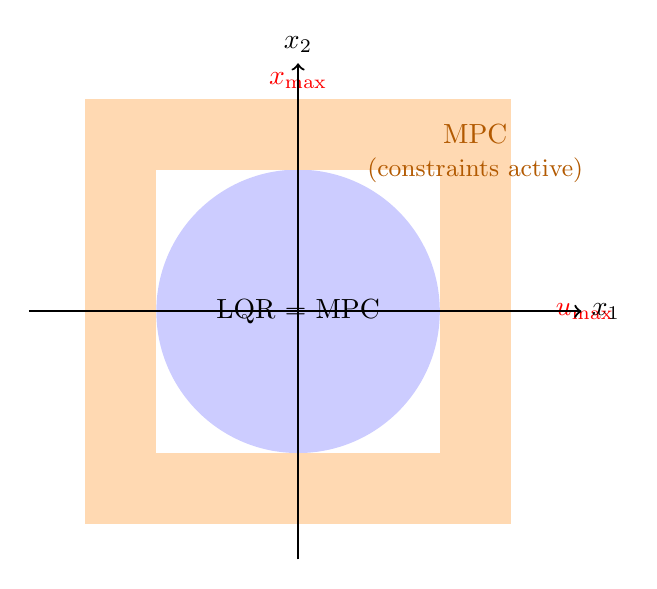
\begin{tikzpicture}[scale=0.9]
    % LQR region (no constraints active)
    \fill[blue!20] (0,0) circle (2);
    \node at (0,0) {LQR = MPC};
    \node[below] at (0,-2.3) {(no constraints active)};

    % Constraint boundary
    \draw[thick, red] (-3.5,0) -- (3.5,0);
    \draw[thick, red] (0,-3) -- (0,3);
    \node[red, right] at (3.5,0) {$u_{\max}$};
    \node[red, above] at (0,3) {$x_{\max}$};

    % MPC-only region
    \fill[orange!30] (-3,-3) rectangle (-2,3);
    \fill[orange!30] (2,-3) rectangle (3,3);
    \fill[orange!30] (-3,2) rectangle (3,3);
    \fill[orange!30] (-3,-3) rectangle (3,-2);

    \node[orange!70!black] at (2.5,2.5) {MPC};
    \node[orange!70!black, below] at (2.5,2.3) {\small (constraints active)};

    % State space axes
    \draw[->, thick] (-3.8,0) -- (4,0) node[right] {$x_1$};
    \draw[->, thick] (0,-3.5) -- (0,3.5) node[above] {$x_2$};
\end{tikzpicture}
\caption{Relationship between MPC and LQR in state space. In the interior region (blue), constraints are inactive and MPC reduces to LQR. Near boundaries (orange), constraints become active and MPC differs from LQR.}
\label{fig:mpc_lqr_regions}
\end{figure}

%==============================================================================
\section{Practical Laboratory: Tank Level Control with Constraints}
\label{sec:lab}
%==============================================================================

\subsection{Objective}

This experiment demonstrates MPC's key advantage: graceful constraint handling. Students will implement both PID and MPC controllers for a cascaded tank system and observe how each handles actuator saturation during large setpoint changes.

\subsection{System Description}

The experimental apparatus consists of two vertically cascaded tanks with a single pump as the actuator.

\begin{figure}[htbp]
\centering
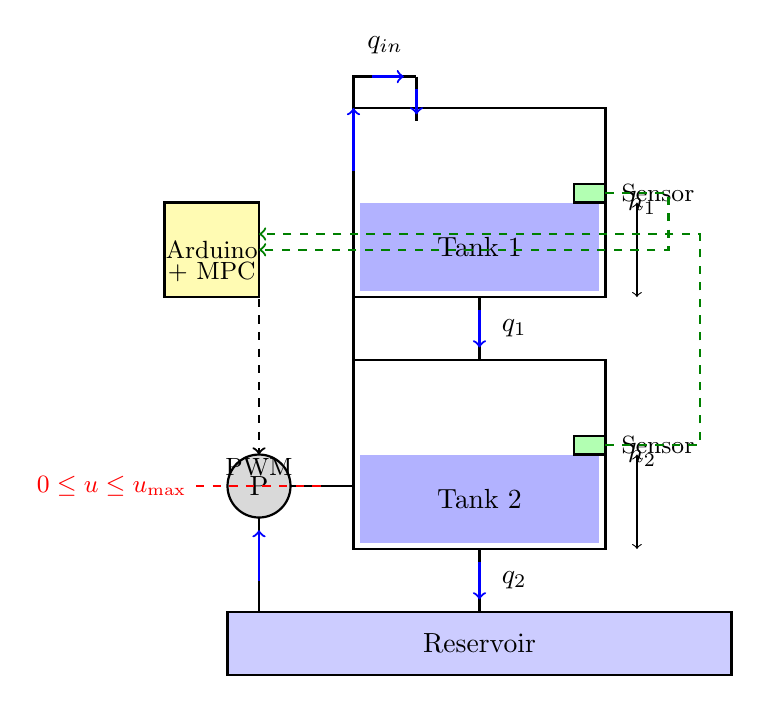
\begin{tikzpicture}[scale=0.8]
    % Lower tank
    \draw[thick] (0,0) rectangle (4,3);
    \fill[blue!30] (0.1,0.1) rectangle (3.9,1.5);
    \node at (2,0.8) {Tank 2};
    \node[right] at (4.2,1.5) {$h_2$};
    \draw[<->] (4.5,0) -- (4.5,1.5);

    % Upper tank
    \draw[thick] (0,4) rectangle (4,7);
    \fill[blue!30] (0.1,4.1) rectangle (3.9,5.5);
    \node at (2,4.8) {Tank 1};
    \node[right] at (4.2,5.5) {$h_1$};
    \draw[<->] (4.5,4) -- (4.5,5.5);

    % Outlet from tank 1 to tank 2
    \draw[thick] (2,4) -- (2,3);
    \draw[->, blue, thick] (2,3.8) -- (2,3.2);
    \node[right] at (2.2,3.5) {$q_1$};

    % Outlet from tank 2
    \draw[thick] (2,0) -- (2,-1);
    \draw[->, blue, thick] (2,-0.2) -- (2,-0.8);
    \node[right] at (2.2,-0.5) {$q_2$};

    % Reservoir
    \fill[blue!20] (-2,-2) rectangle (6,-1);
    \draw[thick] (-2,-2) rectangle (6,-1);
    \node at (2,-1.5) {Reservoir};

    % Pump
    \draw[thick, fill=gray!30] (-1.5,1) circle (0.5);
    \node at (-1.5,1) {P};
    \draw[thick] (-1.5,-1) -- (-1.5,0.5);
    \draw[thick] (-1,1) -- (0,1) -- (0,7.5) -- (1,7.5);
    \draw[->, blue, thick] (-1.5,-0.5) -- (-1.5,0.3);
    \draw[->, blue, thick] (0,6) -- (0,7);
    \draw[->, blue, thick] (0.3,7.5) -- (0.8,7.5);

    % Inlet to tank 1
    \draw[thick] (1,7.5) -- (1,7) -- (1,6.8);
    \draw[->, blue, thick] (1,7.3) -- (1,6.9);
    \node[above] at (0.5,7.7) {$q_{in}$};

    % Level sensors
    \draw[thick, fill=green!30] (3.5,5.5) rectangle (4,5.8);
    \node[right] at (4.1,5.65) {\small Sensor};
    \draw[thick, fill=green!30] (3.5,1.5) rectangle (4,1.8);
    \node[right] at (4.1,1.65) {\small Sensor};

    % Controller
    \draw[thick, fill=yellow!30] (-3,4) rectangle (-1.5,5.5);
    \node at (-2.25,4.75) {\small Arduino};
    \node at (-2.25,4.4) {\small + MPC};

    % Controller connections
    \draw[->, thick, dashed] (-1.5,4.5) -- (-1.5,1.5);
    \draw[->, thick, dashed, green!50!black] (4,5.65) -- (5,5.65) -- (5,4.75) -- (-1.5,4.75);
    \draw[->, thick, dashed, green!50!black] (4,1.65) -- (5.5,1.65) -- (5.5,5) -- (-1.5,5);

    % Annotations
    \node[below] at (-1.5,1.6) {\small PWM};

    % Constraint indicators
    \draw[thick, red, dashed] (-2.5,1) -- (-0.5,1);
    \node[red, left] at (-2.5,1) {\small $0 \leq u \leq u_{\max}$};

\end{tikzpicture}
\caption{Cascaded two-tank system. Water flows from reservoir through pump to Tank 1, drains to Tank 2, and returns to reservoir. The pump can only push water (unidirectional), creating a fundamental input constraint.}
\label{fig:tank_setup}
\end{figure}

\textbf{Key constraint}: The pump can only push water into the system---it cannot pull water out. This creates a hard input constraint: $0 \leq u \leq u_{\max}$.

When the operator requests a rapid decrease in tank level, a PID controller will command negative pump speed (impossible) and saturate at zero, causing integrator windup. MPC, knowing the constraint, will instead plan a trajectory that decreases level by simply reducing inflow and waiting for natural drainage.

\subsection{System Modeling}

\textbf{Physical equations}:

Mass balance for each tank:
\begin{align}
    A_1 \frac{dh_1}{dt} &= q_{in} - q_1 = q_{in} - a_1\sqrt{2gh_1} \\
    A_2 \frac{dh_2}{dt} &= q_1 - q_2 = a_1\sqrt{2gh_1} - a_2\sqrt{2gh_2}
\end{align}

where $A_i$ is tank cross-sectional area, $a_i$ is outlet orifice area, and $g$ is gravitational acceleration.

\textbf{Linearization} around operating point $(h_1^0, h_2^0, q_{in}^0)$:

Define deviation variables: $\tilde{h}_i = h_i - h_i^0$, $\tilde{u} = q_{in} - q_{in}^0$.

The linearized model is:
\begin{equation}
    \begin{bmatrix} \dot{\tilde{h}}_1 \\ \dot{\tilde{h}}_2 \end{bmatrix} =
    \begin{bmatrix} -\frac{1}{T_1} & 0 \\ \frac{1}{T_1} & -\frac{1}{T_2} \end{bmatrix}
    \begin{bmatrix} \tilde{h}_1 \\ \tilde{h}_2 \end{bmatrix} +
    \begin{bmatrix} \frac{K_1}{T_1} \\ 0 \end{bmatrix} \tilde{u}
\end{equation}

where the time constants $T_i = \frac{A_i}{a_i}\sqrt{\frac{2h_i^0}{g}}$ and gain $K_1 = \frac{1}{a_1\sqrt{2gh_1^0}}$ depend on the operating point.

\textbf{Discrete-time model}: Using zero-order hold with sampling time $T_s$:
\begin{equation}
    \state_{k+1} = \mat{A}_d \state_k + \mat{B}_d u_k
\end{equation}

\subsection{Required Components}

\begin{table}[htbp]
\centering
\caption{Bill of Materials for Tank Control Experiment}
\label{tab:tank_bom}
\begin{tabular}{lll}
\toprule
\textbf{Component} & \textbf{Specification} & \textbf{Qty} \\
\midrule
Arduino Mega 2560 & ATmega2560 microcontroller & 1 \\
Water pump & 6-12V DC, 2-5 L/min & 1 \\
Motor driver & L298N or similar & 1 \\
Tanks & 3D printed, $\sim$500 mL each & 2 \\
Ultrasonic sensors & HC-SR04 or waterproof equivalent & 2 \\
Tubing & 8mm ID silicone & 2m \\
Orifice fittings & 3-5mm diameter & 2 \\
Reservoir & Any container $>$2L & 1 \\
Power supply & 12V, 3A & 1 \\
\bottomrule
\end{tabular}
\end{table}

\textbf{3D Printing Notes}: Tank walls should be at least 3mm thick for adequate water resistance. PETG is the recommended material due to its water resistance and food-safe properties. The design should include mounting points for sensors and tubes, and o-ring grooves should be considered for leak-proof fittings. At 0.2mm layer height, expect approximately 4--6 hours of print time per tank.

\subsection{Software Implementation}

\subsubsection{PID Controller with Anti-Windup}

\begin{algorithm}[H]
\caption{PID Controller with Anti-Windup}
\label{alg:pid_tank}
\begin{algorithmic}[1]
\State \textbf{Parameters:} $K_p$, $K_i$, $K_d$, $u_{\min}$, $u_{\max}$
\State \textbf{State variables:} $I \gets 0$ (integral accumulator), $e_{\text{prev}} \gets 0$
\State
\Function{Compute}{$r$, $y$, $\Delta t$} \Comment{$r$ = setpoint, $y$ = measurement}
    \State $e \gets r - y$ \Comment{Compute error}
    \State $P \gets K_p \cdot e$ \Comment{Proportional term}
    \State $I \gets I + K_i \cdot e \cdot \Delta t$ \Comment{Integral term}
    \State $D \gets K_d \cdot (e - e_{\text{prev}}) / \Delta t$ \Comment{Derivative term}
    \State $u \gets P + I + D$ \Comment{Compute raw output}
    \If{$u > u_{\max}$}
        \State $I \gets I - (u - u_{\max})$ \Comment{Anti-windup: reduce integral}
        \State $u \gets u_{\max}$
    \ElsIf{$u < u_{\min}$}
        \State $I \gets I - (u - u_{\min})$ \Comment{Anti-windup: increase integral}
        \State $u \gets u_{\min}$
    \EndIf
    \State $e_{\text{prev}} \gets e$
    \State \Return $u$
\EndFunction
\end{algorithmic}
\end{algorithm}

\subsubsection{Simple MPC Implementation}

For this educational experiment, we implement a simplified MPC that solves the unconstrained problem analytically, then projects the solution onto the constraint set.

\begin{algorithm}[H]
\caption{Simplified MPC for Two-Tank System}
\label{alg:mpc_tank}
\begin{algorithmic}[1]
\State \textbf{Offline Initialization:}
\State \textbf{Input:} System matrices $\mat{A}$, $\mat{B}$; weights $\mat{Q}$, $R$; constraints $u_{\min}$, $u_{\max}$; horizon $N$
\State Compute prediction matrices $\boldsymbol{\mathcal{A}}$, $\boldsymbol{\mathcal{B}}$ from $\mat{A}$, $\mat{B}$, $N$
\State Compute Hessian $H \gets \boldsymbol{\mathcal{B}}^\top \bar{\mat{Q}} \boldsymbol{\mathcal{B}} + \bar{\mat{R}}$
\State Compute linear coefficient matrix $\mat{F} \gets \boldsymbol{\mathcal{B}}^\top \bar{\mat{Q}} \boldsymbol{\mathcal{A}}$
\State
\State \textbf{Online Control Loop:}
\While{system is running}
    \State Read sensor measurements $h_1$, $h_2$
    \State Compute state deviation: $\vect{x} \gets [h_1 - r_1, \, h_2 - r_2]^\top$
    \State Compute linear cost term: $f \gets \mat{F} \cdot \vect{x}$
    \State Compute unconstrained optimum: $u^* \gets -H^{-1} f$
    \State Project onto constraints:
    \If{$u^* < u_{\min}$}
        \State $u^* \gets u_{\min}$
    \ElsIf{$u^* > u_{\max}$}
        \State $u^* \gets u_{\max}$
    \EndIf
    \State Apply control signal $u^*$ to pump
    \State Log data: $h_1$, $h_2$, $u^*$, setpoints
    \State Wait for next sampling instant
\EndWhile
\end{algorithmic}
\end{algorithm}

\subsection{Experimental Procedure}

\subsubsection{Part 1: System Identification}

Begin by filling the reservoir and establishing steady-state operation at mid-level in both tanks. Apply step changes in pump PWM, for example from 100 to 150, and record the resulting tank level responses over time. Using the recorded data, fit first-order-plus-delay models to the step responses. From these fitted models, extract the time constants $T_1$ and $T_2$ along with the system gains for use in the MPC prediction model.

\subsubsection{Part 2: PID Control Experiment}

Tune the PID controller to achieve acceptable step response performance at the nominal operating point. Command a large positive setpoint change to request a level increase, and observe that while the pump saturates at its maximum value, the system recovers reasonably. Next, command a large negative setpoint change to request a level decrease. Observe that the pump saturates at zero since it cannot provide negative flow, causing the integrator to wind up. Record the overshoot, settling time, and any constraint violations for later comparison with MPC.

\subsubsection{Part 3: MPC Control Experiment}

Configure the MPC controller with tuning parameters that target the same response speed as the PID controller. Repeat the large positive setpoint change and observe that MPC may preemptively limit the pump rate to avoid later saturation. When repeating the large negative setpoint change, observe that MPC reduces the pump command to its minimum value without attempting negative values, instead planning a feasible descent trajectory that respects the physical constraint. Compare the performance metrics from MPC to those recorded for PID control.

\subsection{Expected Results}

\begin{figure}[htbp]
\centering
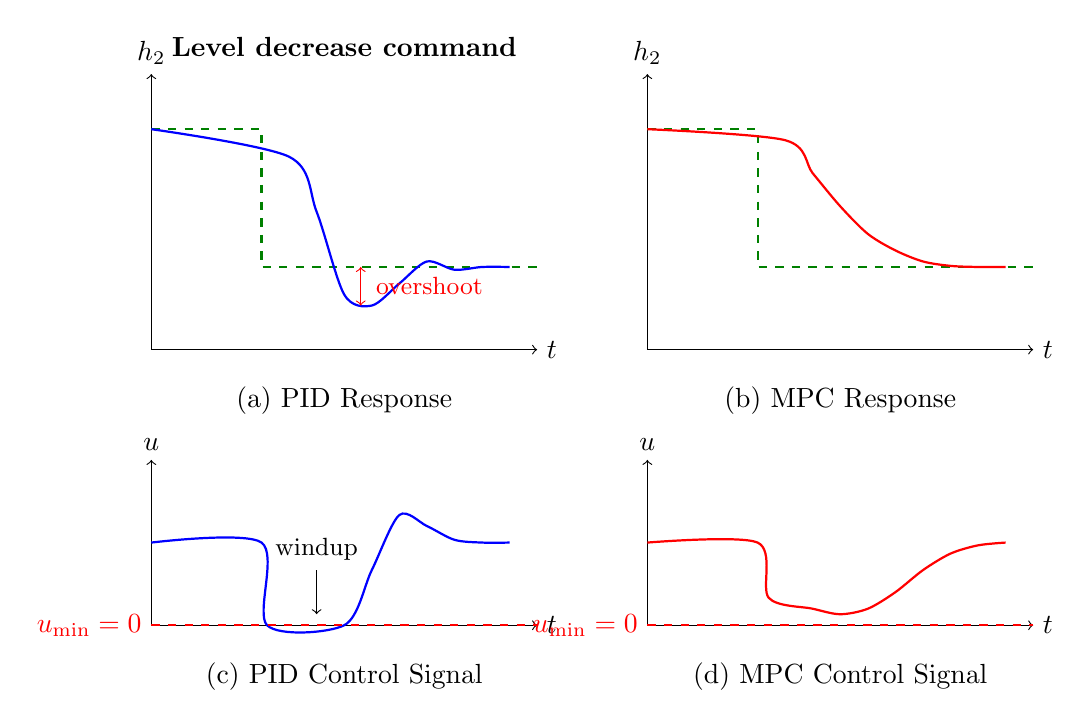
\begin{tikzpicture}[scale=0.7]
    % PID Response (left plot)
    \begin{scope}
        \draw[->] (0,0) -- (7,0) node[right] {$t$};
        \draw[->] (0,0) -- (0,5) node[above] {$h_2$};

        % Setpoint
        \draw[thick, dashed, green!50!black] (0,4) -- (2,4) -- (2,1.5) -- (7,1.5);

        % PID response with overshoot
        \draw[thick, blue] plot[smooth] coordinates
            {(0,4) (2.5,3.5) (3,2.5) (3.5,1) (4,0.8) (4.5,1.2) (5,1.6) (5.5,1.45) (6,1.5) (6.5,1.5)};

        % Undershoot annotation
        \draw[<->, red] (3.8,0.8) -- (3.8,1.5);
        \node[red, right] at (3.9,1.15) {\small overshoot};

        \node[below] at (3.5,-0.5) {(a) PID Response};
        \node at (3.5,5.5) {\textbf{Level decrease command}};
    \end{scope}

    % MPC Response (right plot)
    \begin{scope}[xshift=9cm]
        \draw[->] (0,0) -- (7,0) node[right] {$t$};
        \draw[->] (0,0) -- (0,5) node[above] {$h_2$};

        % Setpoint
        \draw[thick, dashed, green!50!black] (0,4) -- (2,4) -- (2,1.5) -- (7,1.5);

        % MPC response - smooth approach
        \draw[thick, red] plot[smooth] coordinates
            {(0,4) (2.5,3.8) (3,3.2) (3.5,2.6) (4,2.1) (4.5,1.8) (5,1.6) (5.5,1.52) (6,1.5) (6.5,1.5)};

        \node[below] at (3.5,-0.5) {(b) MPC Response};
    \end{scope}

    % Control signals
    \begin{scope}[yshift=-5cm]
        \draw[->] (0,0) -- (7,0) node[right] {$t$};
        \draw[->] (0,0) -- (0,3) node[above] {$u$};

        % PID control - saturates at 0, then overshoots
        \draw[thick, blue] plot[smooth] coordinates
            {(0,1.5) (2,1.5) (2.1,0) (3.5,0) (4,1) (4.5,2) (5,1.8) (5.5,1.55) (6,1.5) (6.5,1.5)};

        % Saturation line
        \draw[thick, red, dashed] (0,0) -- (7,0);
        \node[red, left] at (0,0) {$u_{\min}=0$};

        % Windup annotation
        \draw[<-] (3,0.2) -- (3,1) node[above] {\small windup};

        \node[below] at (3.5,-0.5) {(c) PID Control Signal};
    \end{scope}

    \begin{scope}[xshift=9cm, yshift=-5cm]
        \draw[->] (0,0) -- (7,0) node[right] {$t$};
        \draw[->] (0,0) -- (0,3) node[above] {$u$};

        % MPC control - respects constraint, smooth
        \draw[thick, red] plot[smooth] coordinates
            {(0,1.5) (2,1.5) (2.2,0.5) (3,0.3) (3.5,0.2) (4,0.3) (4.5,0.6) (5,1) (5.5,1.3) (6,1.45) (6.5,1.5)};

        % Saturation line
        \draw[thick, red, dashed] (0,0) -- (7,0);
        \node[red, left] at (0,0) {$u_{\min}=0$};

        \node[below] at (3.5,-0.5) {(d) MPC Control Signal};
    \end{scope}
\end{tikzpicture}
\caption{Comparison of PID and MPC for large level decrease. PID saturates at $u=0$, causing integrator windup and subsequent overshoot. MPC anticipates the constraint and plans a feasible trajectory, achieving monotonic convergence.}
\label{fig:pid_vs_mpc}
\end{figure}

\begin{table}[htbp]
\centering
\caption{Expected Performance Comparison}
\label{tab:performance}
\begin{tabular}{lcc}
\toprule
\textbf{Metric} & \textbf{PID} & \textbf{MPC} \\
\midrule
Rise time (level increase) & Similar & Similar \\
Settling time (level decrease) & Longer & Shorter \\
Overshoot (level decrease) & 10-20\% & $<$5\% \\
Constraint satisfaction & Violations & Always satisfied \\
Control smoothness & Oscillatory & Smooth \\
\bottomrule
\end{tabular}
\end{table}

\subsection{Discussion Questions}

\begin{enumerate}
    \item Why does MPC produce smoother control signals than PID in constrained situations?
    \item How would increasing the MPC horizon $N$ affect performance and computation time?
    \item What modifications would be needed if the pump could also pull water (bidirectional)?
    \item How would you handle a constraint on maximum tank level (overflow prevention)?
\end{enumerate}

%==============================================================================
\section{Worked Examples}
\label{sec:examples}
%==============================================================================

\begin{examplebox}[Setting Up MPC Matrices for a Double Integrator]
\textbf{Problem}: A double integrator system (mass under force control) has dynamics:
\begin{equation}
    \ddot{x} = u
\end{equation}
Set up the MPC prediction matrices for a horizon of $N=3$ with sampling time $T_s = 0.1$ s.

\textbf{Solution}:

\textit{Step 1}: Discretize the continuous-time system.

State vector: $\state = [x, \dot{x}]^\top$

Continuous-time matrices:
\begin{equation}
    \mat{A}_c = \begin{bmatrix} 0 & 1 \\ 0 & 0 \end{bmatrix}, \quad
    \mat{B}_c = \begin{bmatrix} 0 \\ 1 \end{bmatrix}
\end{equation}

Discrete-time matrices (using $\mat{A}_d = e^{\mat{A}_c T_s}$, $\mat{B}_d = \int_0^{T_s} e^{\mat{A}_c \tau} d\tau \mat{B}_c$):
\begin{equation}
    \mat{A} = \begin{bmatrix} 1 & 0.1 \\ 0 & 1 \end{bmatrix}, \quad
    \mat{B} = \begin{bmatrix} 0.005 \\ 0.1 \end{bmatrix}
\end{equation}

\textit{Step 2}: Build the prediction matrices.

\begin{equation}
    \boldsymbol{\mathcal{A}} = \begin{bmatrix} \mat{A} \\ \mat{A}^2 \\ \mat{A}^3 \end{bmatrix} =
    \begin{bmatrix}
        1 & 0.1 \\
        0 & 1 \\
        1 & 0.2 \\
        0 & 1 \\
        1 & 0.3 \\
        0 & 1
    \end{bmatrix}
\end{equation}

\begin{equation}
    \boldsymbol{\mathcal{B}} = \begin{bmatrix}
        \mat{B} & \mat{0} & \mat{0} \\
        \mat{A}\mat{B} & \mat{B} & \mat{0} \\
        \mat{A}^2\mat{B} & \mat{A}\mat{B} & \mat{B}
    \end{bmatrix} =
    \begin{bmatrix}
        0.005 & 0 & 0 \\
        0.1 & 0 & 0 \\
        0.015 & 0.005 & 0 \\
        0.2 & 0.1 & 0 \\
        0.03 & 0.015 & 0.005 \\
        0.3 & 0.2 & 0.1
    \end{bmatrix}
\end{equation}

\textit{Step 3}: Form the Hessian matrix.

With $\mat{Q} = \text{diag}(1, 0.1)$ (penalize position more than velocity) and $\mat{R} = 0.01$:
\begin{equation}
    \bar{\mat{Q}} = \text{diag}(\mat{Q}, \mat{Q}, \mat{Q}) \in \Real^{6 \times 6}
\end{equation}
\begin{equation}
    \bar{\mat{R}} = \text{diag}(0.01, 0.01, 0.01) \in \Real^{3 \times 3}
\end{equation}
\begin{equation}
    \mat{H} = \boldsymbol{\mathcal{B}}^\top \bar{\mat{Q}} \boldsymbol{\mathcal{B}} + \bar{\mat{R}}
\end{equation}

Computing $\mat{H}$ (showing structure):
\begin{equation}
    \mat{H} = \begin{bmatrix}
        0.0116 & 0.0065 & 0.0031 \\
        0.0065 & 0.0113 & 0.0063 \\
        0.0031 & 0.0063 & 0.0110
    \end{bmatrix}
\end{equation}

The off-diagonal coupling shows how future controls affect the current optimal decision.
\end{examplebox}

\begin{examplebox}[QP Formulation with Input Constraints]

\textbf{Problem}: For the double integrator from the previous example, formulate the complete QP with constraints $-1 \leq u_k \leq 1$ for all $k$.

\textbf{Solution}:

The optimization variable is:
\begin{equation}
    \mathbf{U} = \begin{bmatrix} u_0 \\ u_1 \\ u_2 \end{bmatrix}
\end{equation}

\textit{Cost function}:
\begin{equation}
    J = \frac{1}{2} \mathbf{U}^\top \mat{H} \mathbf{U} + \vect{f}^\top \mathbf{U}
\end{equation}
where $\vect{f} = \boldsymbol{\mathcal{B}}^\top \bar{\mat{Q}} \boldsymbol{\mathcal{A}} \state_0$ depends on current state $\state_0$.

\textit{Constraints}:

Upper bounds: $u_i \leq 1$, or $\mat{I} \mathbf{U} \leq \vect{1}$

Lower bounds: $u_i \geq -1$, or $-\mat{I} \mathbf{U} \leq \vect{1}$

Combined inequality form:
\begin{equation}
    \begin{bmatrix} \mat{I}_3 \\ -\mat{I}_3 \end{bmatrix} \mathbf{U} \leq
    \begin{bmatrix} 1 \\ 1 \\ 1 \\ 1 \\ 1 \\ 1 \end{bmatrix}
\end{equation}

\textit{Complete QP}:
\begin{equation}
\boxed{
\begin{aligned}
    \min_{\mathbf{U}} \quad & \frac{1}{2} \mathbf{U}^\top
    \begin{bmatrix} 0.0116 & 0.0065 & 0.0031 \\ 0.0065 & 0.0113 & 0.0063 \\ 0.0031 & 0.0063 & 0.0110 \end{bmatrix}
    \mathbf{U} + \vect{f}^\top \mathbf{U} \\
    \text{s.t.} \quad & -\vect{1} \leq \mathbf{U} \leq \vect{1}
\end{aligned}
}
\end{equation}
\end{examplebox}

\subsection{Example 3: Comparing Unconstrained MPC to LQR}

\textbf{Problem}: For the system $\state_{k+1} = \begin{bmatrix} 0.9 & 0.1 \\ 0 & 0.8 \end{bmatrix} \state_k + \begin{bmatrix} 0.05 \\ 0.1 \end{bmatrix} u_k$ with $\mat{Q} = \mat{I}_2$, $\mat{R} = 1$:

(a) Compute the infinite-horizon LQR gain
(b) Compute the MPC control for horizon $N=20$ at state $\state_0 = [1, 0]^\top$
(c) Compare the first control actions

\textbf{Solution}:

\textit{(a) LQR Solution}:

Solve the discrete algebraic Riccati equation (DARE):
\begin{equation}
    \mat{P} = \mat{Q} + \mat{A}^\top \mat{P} \mat{A} - \mat{A}^\top \mat{P} \mat{B} (\mat{R} + \mat{B}^\top \mat{P} \mat{B})^{-1} \mat{B}^\top \mat{P} \mat{A}
\end{equation}

Numerical solution (e.g., using MATLAB's \texttt{dare}):
\begin{equation}
    \mat{P} = \begin{bmatrix} 2.76 & 1.32 \\ 1.32 & 3.18 \end{bmatrix}
\end{equation}

LQR gain:
\begin{equation}
    \mat{K} = (\mat{R} + \mat{B}^\top \mat{P} \mat{B})^{-1} \mat{B}^\top \mat{P} \mat{A} = \begin{bmatrix} 0.183 & 0.323 \end{bmatrix}
\end{equation}

At $\state_0 = [1, 0]^\top$:
\begin{equation}
    u_{\text{LQR}} = -\mat{K} \state_0 = -0.183
\end{equation}

\textit{(b) MPC Solution with $N=20$}:

Set terminal cost $\mat{P}$ equal to the LQR cost matrix from part (a).

Using numerical QP solver with $N=20$ horizon:
\begin{equation}
    u_{\text{MPC}}^* = -0.183
\end{equation}

\textit{(c) Comparison}:
\begin{equation}
    u_{\text{LQR}} = u_{\text{MPC}}^* = -0.183
\end{equation}

The solutions match exactly! This confirms that unconstrained MPC with appropriate terminal cost converges to LQR as $N$ increases.

\hfill $\blacksquare$

\subsection{Example 4: Effect of Prediction Horizon Length}

\textbf{Problem}: For the double integrator system, analyze how the MPC control action at $\state_0 = [1, 0]^\top$ varies with horizon length $N = 1, 2, 5, 10, 20$.

\textbf{Solution}:

Using $\mat{Q} = \text{diag}(1, 0.1)$, $\mat{R} = 0.01$, and terminal cost $\mat{P} = \mat{Q}$ (suboptimal choice for illustration):

\begin{table}[htbp]
\centering
\begin{tabular}{ccc}
\toprule
$N$ & $u_0^*$ & Cost $J$ \\
\midrule
1 & -0.42 & 1.002 \\
2 & -0.58 & 0.995 \\
5 & -0.71 & 0.982 \\
10 & -0.79 & 0.971 \\
20 & -0.85 & 0.963 \\
$\infty$ (LQR) & -0.91 & 0.958 \\
\bottomrule
\end{tabular}
\end{table}

\textbf{Observations}: Short horizons such as $N=1$ or $N=2$ produce less aggressive control because the controller ``doesn't see'' far enough into the future. As $N$ increases, the control action approaches the LQR solution, and the cost decreases due to greater optimization freedom. However, there are diminishing returns: $N=10$ captures most of the benefit, suggesting that extremely long horizons may not justify the additional computational cost.

\textbf{Practical guideline}: Choose $N$ such that open-loop predictions extend beyond the system's dominant time constant.

\hfill $\blacksquare$

\subsection{Example 5: MPC for Setpoint Tracking}

\textbf{Problem}: Modify the MPC formulation to track a non-zero setpoint $\state_{\text{ref}}$, $u_{\text{ref}}$ for the system:
\begin{equation}
    \state_{k+1} = \begin{bmatrix} 1 & 0.1 \\ 0 & 0.9 \end{bmatrix} \state_k + \begin{bmatrix} 0 \\ 0.1 \end{bmatrix} u_k
\end{equation}
where we want to track $\state_{\text{ref}} = [5, 0]^\top$ (position of 5, zero velocity).

\textbf{Solution}:

\textit{Step 1}: Find steady-state input.

At steady state: $\state_{\text{ref}} = \mat{A} \state_{\text{ref}} + \mat{B} u_{\text{ref}}$
\begin{equation}
    \begin{bmatrix} 5 \\ 0 \end{bmatrix} = \begin{bmatrix} 1 & 0.1 \\ 0 & 0.9 \end{bmatrix} \begin{bmatrix} 5 \\ 0 \end{bmatrix} + \begin{bmatrix} 0 \\ 0.1 \end{bmatrix} u_{\text{ref}}
\end{equation}

From the second row: $0 = 0 + 0.1 u_{\text{ref}} \Rightarrow u_{\text{ref}} = 0$

\textit{Step 2}: Transform to deviation coordinates.

Define: $\tilde{\state}_k = \state_k - \state_{\text{ref}}$, $\tilde{u}_k = u_k - u_{\text{ref}}$

The dynamics in deviation coordinates:
\begin{equation}
    \tilde{\state}_{k+1} = \mat{A} \tilde{\state}_k + \mat{B} \tilde{u}_k
\end{equation}

\textit{Step 3}: Apply standard MPC to deviation system.

Cost function (penalizes deviation from setpoint):
\begin{equation}
    J = \sum_{i=0}^{N-1} \left( \tilde{\state}_{k+i}^\top \mat{Q} \tilde{\state}_{k+i} + \tilde{u}_{k+i}^\top \mat{R} \tilde{u}_{k+i} \right) + \tilde{\state}_{k+N}^\top \mat{P} \tilde{\state}_{k+N}
\end{equation}

Constraints transform accordingly:
\begin{equation}
    u_{\min} - u_{\text{ref}} \leq \tilde{u}_k \leq u_{\max} - u_{\text{ref}}
\end{equation}

\textit{Step 4}: Solve QP and convert back.

After solving for optimal $\tilde{u}_k^*$:
\begin{equation}
    u_k^* = \tilde{u}_k^* + u_{\text{ref}}
\end{equation}

This procedure ensures the controller drives $\state \to \state_{\text{ref}}$ with $u \to u_{\text{ref}}$.

\hfill $\blacksquare$

%==============================================================================
\section{MPC Block Diagram and Architecture}
\label{sec:architecture}
%==============================================================================

\begin{figure}[htbp]
\centering
\begin{tikzpicture}[scale=0.85, auto, node distance=2cm, >=latex]
    % Blocks
    \node[draw, rectangle, minimum width=3cm, minimum height=1.5cm, fill=blue!20] (mpc) {MPC Optimizer};
    \node[draw, rectangle, minimum width=2.5cm, minimum height=1cm, below=1.5cm of mpc, fill=green!20] (plant) {Plant $G(s)$};
    \node[draw, rectangle, minimum width=2.5cm, minimum height=1cm, left=2cm of plant, fill=yellow!20] (model) {Model $\hat{G}(s)$};
    \node[draw, circle, right=1.5cm of plant, inner sep=2pt] (sum1) {$+$};
    \node[draw, rectangle, minimum width=2cm, minimum height=0.8cm, below=1cm of plant, fill=orange!20] (observer) {State Observer};

    % Input/Output
    \node[left=2.5cm of mpc] (ref) {$r_k$};
    \node[right=2cm of sum1] (output) {$y_k$};
    \node[above=0.8cm of sum1] (dist) {$d_k$};

    % Connections
    \draw[->] (ref) -- node[above] {setpoint} (mpc);
    \draw[->] (mpc) -- node[right] {$u_k^*$} ++(0,-1) -| (plant.north);
    \draw[->] (mpc) -- node[left, pos=0.3] {$u_k^*$} ++(0,-1) -- ++(-2,0) -- (model.north);
    \draw[->] (plant) -- (sum1);
    \draw[->] (sum1) -- (output);
    \draw[->] (dist) -- node[right] {disturbance} (sum1);

    % Feedback
    \coordinate (fb1) at ($(sum1.east)+(0.5,0)$);
    \draw[->] (fb1) |- (observer.east);
    \draw[->] (observer) -- ++(-4,0) |- (mpc.west);

    % Model prediction feedback
    \draw[->] (model.south) -- ++(0,-0.5) -| node[below, pos=0.25] {$\hat{y}_{k+i|k}$} (observer.west);

    % Annotations
    \node[above=0.3cm of mpc] {\textbf{MPC Controller}};
    \draw[dashed, thick, gray] (-4.5,-5) rectangle (2,2);

    % Constraint annotation
    \node[draw, rectangle, dashed, red, minimum width=1.5cm, right=0.3cm of mpc, anchor=west] (const) {\small Constraints};
    \draw[->, red] (const) -- (mpc);

\end{tikzpicture}
\caption{MPC control system architecture. The optimizer receives the setpoint, current state estimate, and constraints, then solves the QP to produce the optimal control sequence. Only the first control action is applied; the process repeats at the next sample.}
\label{fig:mpc_architecture}
\end{figure}

%==============================================================================
\section{Chapter Summary}
\label{sec:summary}
%==============================================================================

This chapter developed Model Predictive Control from industrial origins to mathematical rigor.

\textbf{Historical Context.} MPC emerged from 1970s petrochemical control challenges. Shell's DMC and Richalet's MPHC provided practical algorithms before complete theoretical understanding existed. The key insight was using process models for prediction and optimization for constraint handling.

\textbf{Modern Applications.} MPC now spans chemical processes, autonomous vehicles, building systems, and robotics---any domain requiring constraint-aware trajectory optimization.

\textbf{Mathematical Foundation.} MPC solves finite-horizon optimal control problems at each sampling instant. The approach combines a prediction model ($\state_{k+1} = \mat{A}\state_k + \mat{B}u_k$) with a cost function applying quadratic penalties on states and inputs. Constraints on inputs, states, and terminal conditions are handled explicitly. The receding horizon strategy solves the optimization, applies only the first input, and repeats at each sampling instant.

\textbf{QP Formulation.} Eliminating state predictions converts MPC to standard quadratic programming:
\begin{equation*}
    \min_{\mathbf{U}} \frac{1}{2}\mathbf{U}^\top\mat{H}\mathbf{U} + \vect{f}^\top\mathbf{U} \quad \text{s.t.} \quad \mat{G}\mathbf{U} \leq \vect{w}
\end{equation*}

\textbf{Stability.} Terminal cost or constraints ensure closed-loop stability. With appropriate terminal cost, unconstrained MPC equals LQR.

\textbf{Practical Implementation.} The tank-level experiment demonstrated MPC's graceful constraint handling compared to PID's windup problems.

\begin{tcolorbox}[colback=yellow!10!white,colframe=orange!75!black,title=Key Takeaway,sharp corners]
Model Predictive Control transforms control from reaction to anticipation. By predicting future behavior and optimizing over horizons while respecting constraints, MPC achieves performance impossible with classical feedback alone. The computational cost---solving an optimization at each step---is the price of this capability, now affordable for most applications thanks to modern processors.
\end{tcolorbox}

\newpage
%==============================================================================
\section{Exercises}
\label{sec:exercises}
%==============================================================================

\subsection{Conceptual Exercises}

\begin{exercise}
Explain why MPC re-solves the optimization problem at every time step rather than executing the entire precomputed control sequence.
\end{exercise}

\begin{exercise}
A colleague claims ``MPC is just optimal control, nothing new.'' Explain what distinguishes MPC from classical optimal control theory.
\end{exercise}

\begin{exercise}
Why does MPC require positive definite $\mat{R}$ but only positive semi-definite $\mat{Q}$?
\end{exercise}

\begin{exercise}
What happens to the MPC solution if the prediction model is perfect versus imperfect?
\end{exercise}

\subsection{Computational Exercises}

\begin{exercise}
For the system $\state_{k+1} = 0.9\state_k + 0.5u_k$ (scalar), with $Q=1$, $R=0.1$, $N=3$:
\begin{enumerate}
    \item Compute the prediction matrices $\boldsymbol{\mathcal{A}}$ and $\boldsymbol{\mathcal{B}}$
    \item Form the Hessian $\mat{H}$
    \item Find the unconstrained optimal control sequence for $\state_0 = 1$
\end{enumerate}
\end{exercise}

\begin{exercise}
Using the system from the previous exercise, add input constraint $|u_k| \leq 0.5$. Show how the constraint affects the solution.
\end{exercise}

\begin{exercise}
For a double integrator with $T_s = 0.1$ s, design MPC parameters ($N$, $\mat{Q}$, $\mat{R}$) to achieve settling time approximately 1 second with input constraint $|u| \leq 10$.
\end{exercise}

\begin{exercise}
Prove that the Hessian matrix $\mat{H} = \boldsymbol{\mathcal{B}}^\top\bar{\mat{Q}}\boldsymbol{\mathcal{B}} + \bar{\mat{R}}$ is positive definite when $\mat{R} \succ 0$.
\end{exercise}

\subsection{Analysis Exercises}

\begin{exercise}
Consider MPC with horizon $N=1$ (one step ahead). Show that this reduces to a simple state feedback law. What is the feedback gain?
\end{exercise}

\begin{exercise}
For a marginally stable system ($\mat{A}$ has eigenvalues on the unit circle), explain why terminal constraints are particularly important for MPC stability.
\end{exercise}

\begin{exercise}
Derive the relationship between MPC and LQR when no constraints are active. Under what conditions are they identical?
\end{exercise}

\subsection{Implementation Exercises}

\begin{exercise}
Implement MPC in MATLAB/Python for a DC motor position control system. Compare performance with PID for:
\begin{enumerate}
    \item Nominal step response
    \item Step response with actuator saturation
    \item Disturbance rejection
\end{enumerate}
\end{exercise}

\begin{exercise}
Extend the tank-level MPC to include a constraint on maximum rate of change of pump speed (slew rate limiting).
\end{exercise}

\begin{exercise}
Implement an MPC controller for a simulated quadrotor hover task with thrust limits.
\end{exercise}

%==============================================================================
\section*{Further Reading}
\addcontentsline{toc}{section}{Further Reading}
%==============================================================================

For an excellent introduction with practical emphasis, see J. M. Maciejowski's \textit{Predictive Control with Constraints} (Prentice Hall, 2002). A comprehensive theoretical treatment is provided by J. B. Rawlings and D. Q. Mayne in \textit{Model Predictive Control: Theory and Design} (Nob Hill Publishing, 2009). The classic survey paper by C. E. Garcia, D. M. Prett, and M. Morari, ``Model Predictive Control: Theory and Practice---A Survey,'' published in \textit{Automatica}, vol.~25, no.~3, pp.~335--348 (1989), remains an essential reference. For an overview of industrial applications, consult S. J. Qin and T. A. Badgwell's ``A Survey of Industrial Model Predictive Control Technology'' in \textit{Control Engineering Practice}, vol.~11, no.~7, pp.~733--764 (2003). A modern treatment including hybrid systems can be found in F. Borrelli, A. Bemporad, and M. Morari's \textit{Predictive Control for Linear and Hybrid Systems} (Cambridge University Press, 2017).

